\section{Zielsetzung}
Ziel des Versuchs ist die Bestimmung der Zusammensetzung eines Würfels, der sich aus 27 Einheitswürfeln verschiedener Materialien zusammensetzt.
Dazu wird die Tomographie verwendet, welche ein bildgebendes Verfahren ist.


\section{Theorie}
Bei der Tomographie durchdringt Strahlung die Materie, die untersucht werden soll und wird durch die Wechselwirkung mit der Materie abgeschwächt. Die Abschwächung ist materialabhängig, sodass durch Messung der
Intensität auf die Zusammensetzung des untersuchten Objekts geschlossen werden kann. Durch mehrfache Messung der selben Schicht aus verschiedenen Richtungen werden verschiedene Projektionen erzeugt, die zu einem
zweidimensionalen Abbild des Objekts zusammengesetzt werden können.

\subsection{Grundlagen}
Als $\gamma$-Strahlungsquelle wird ${}^{137}\text{Cs}$ verwendet, dessen radioaktiver Zerfall zu ${}^{137}Ba$ in Abbildung \ref{fig:zerfall} dargestellt ist.
Das ${}^{137}\text{Cs}$ zerfällt mit einer Wahrscheinlichkeit von $\SI{5.4}{\%}$ direkt in den Grundzustand des ${}^{137}Ba$ und zerfällt sonst erst
in einen angeregten Bariumkern, welcher unter Aussendung eines Photons mit der Energie von $\SI{662}{keV}$ in den Grundzustand fällt.

\begin{figure}
  \centering
  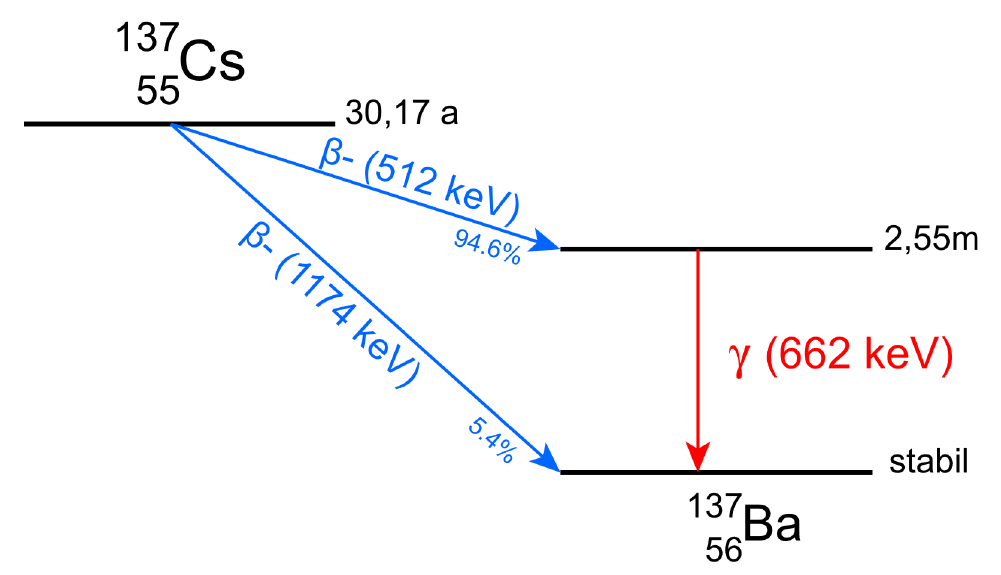
\includegraphics[scale=0.4]{graphics/Zerfall.png}
  \caption{Zerfallsschema von ${}^{137}\text{Cs}$\cite{zerfall}.}
  \label{fig:zerfall}
\end{figure}

Die Wechselwirkung der $\gamma$-Strahlung mit Materie setzt sich im Wesentlichen aus drei verschiedenen Prozessen zusammen: Photoeffekt, Compton-Effekt und Paarbildung.

Beim Photoeffekt gibt das Photon seine gesamte Energie an ein Hüllenelektron eines Atoms ab und wird dabei absorbiert. Das Elektron wird dabei aus seiner
Bindung gelöst und erhält die gesamte Photonenenergie abzüglich der Bindungsenergie. Deshalb tritt der Effekt erst bei $E_\gamma > E_\text{B}$ auf.

Der Compton-Effekt beschreibt die inelastische Streuung eines Photons an einem Elektron, bei der das Photon nur einen Teil seiner Energie abgibt und nicht
absorbiert wird. Bis zu einer Photonenenergie von $\SI{100}{keV}$ dominiert der Photoeffekt und im Bereich $\SI{100}{keV} - \SI{10}{MeV}$ der
Compton-Effekt.

Bei der Paarbildung zerfällt ein Photon im Coulomb-Feld eines Atomkerns in ein Elektron und ein Positron. Dabei wird die Energie des Photons größtenteils in die Ruheenergie
und die kinetische Energie des Elektrons und des Positrons umgewandelt. Das bedeutet, dass die Energie des Photons aufgrund der Energieerhaltung mindestens der Summe der
Ruheenergien ($2m_\text{e}c^2 = \SI{1.02}{MeV}$) entsprechen muss, damit die Paarbildung stattfinden kann. Bei der Verwendung von ${}^{137}\text{Cs}$ spielt die Paarbildung
keine Rolle, da die Strahlung nicht genug Energie besitzt.

Durch Überlagerung der verschiedenen Effekte entsteht insgesamt ein exponentieller Zusammenhang zwischen der Intensität der Strahlung und dem
Absorptionskoeffizient $\mu$ des jeweiligen Materials, welches die Strahlung durchdringt:
\begin{equation}
  \bar{I} = I_0 \exp\left( \sum_i \mu_i d_i \right)
  \label{eq:N}
\end{equation}
Dabei ist $\bar{I}$ die abgeschwächte Intensität, $I_0$ die Anfangintensität und die $d_i$ die Dicke des Materials in Strahlrichtung.

\subsection{Bestimmung der Absorptionskoeffizienten}
Nach Umstellen der Gleichung \eqref{eq:N} zu
\begin{equation}
  \sum_i\mu_i d_i = \ln\left(\frac{I_0}{\bar{I}_j}\right)
\end{equation}
lässt sich diese in Matrixform schreiben:
\begin{equation}
  A\cdot\vec{\mu} = \vec{I}
  \label{eqn:1}
\end{equation}
Der Vektor $\vec{\mu}$ enthält dabei sämtliche Absorptionskoeffizienten der Materialien innerhalb des untersuchten Objekts und der Vektor $\vec{I}$ die Anfangsintensität und die jeweiligen abgeschwächten
Intensitäten für die verschiedenen gewählten Strahlengänge. Die Matrix $A$ enthält die Informationen über die Dicken der jeweiligen Materialien in Strahlrichtung. Für eine Schicht des Objekts, die aus
n elementaren Materialien besteht, ist die Matrix für $m$ Messungen $n\times m$-dimensional. Damit das Gleichungssystem lösbar ist, müssen mindestens $n$
Messungen gemacht werden. Da der Würfel jedoch nicht ganz exakt im Strahlengang ausgerichtet werden kann, werden deutlich mehr als $n$ Messungen vorgenommen, sodass ein
überbestimmtes Gleichungssystem entsteht.

Durch Nutzung der Methode der kleinsten Quadrate lassen sich die unterschiedlichen Unsicherheiten auf die gemessenen Werte von $\vec{I}$ in der Gleichung \ref{eqn:1} berücksichtigen. Dies führt zu der Form
\begin{gather}
  WA\cdot\vec{\mu}=W\vec{I} \\
  \intertext{mit der Gewichtungsmatrix}
  W=V[I]^{-1}
  \label{eqn:gewicht}
\end{gather}
Durch Umstellen dieser Formel ergibt sich nun für $\vec{\mu}$
\begin{equation}
  \vec{\mu}=\left(A^TWA\right)^{-1}\left(A^TW\vec{I}\right)
\end{equation}
mit den Unsicherheiten
\begin{equation}
  V[\mu]=\left(A^TWA\right)^{-1}
  \label{eqn:mu}
\end{equation}
